\subsection{Final 2024 held-out evaluation}
The selected pipeline was evaluated on 6,374,476 valid 2024 base windows,
corresponding to 38,246,856 threshold-expanded rows.
Table~\ref{tab:test} reports per-threshold support, probability scores and
F1; Table~\ref{tab:operating-point} reports precision and recall at the fixed
0.5 probability cutoff.

\begin{table}[htbp]
\centering\scriptsize
\caption{Held-out 2024 support, discrimination, probability error and F1 at
the six primary thresholds. Every threshold uses the same 6,374,476 prediction
times. F1 uses a fixed probability cutoff of 0.5. PR-AUC is Spark's 1,000-bin
evaluator result. ROC-AUC was recomputed locally from saved held-out scores
using \texttt{roc\_auc\_score}~\cite{sklearnroc}. Paired values are
climatology / final PAVA.}
\label{tab:test}
\begin{tabular}{r r r r r r r r}
\toprule
\shortstack{Threshold\\mm} &
\shortstack{Positive\\support} &
\shortstack{Prevalence\\(\%)} &
\shortstack{PR-AUC\\clim. / PAVA} &
\shortstack{ROC-AUC\\clim. / PAVA} &
\shortstack{Brier\\clim. / PAVA} &
F1 \\
\midrule
0.2 & 309,678 & 4.86 & 0.0986 / 0.6618 & 0.5000 / 0.9036 & 0.04520 / 0.02520 & 0.6114 \\
0.5 & 231,071 & 3.62 & 0.0732 / 0.6345 & 0.5000 / 0.9049 & 0.03436 / 0.01958 & 0.6161 \\
1.0 & 163,790 & 2.57 & 0.0529 / 0.5825 & 0.5000 / 0.9029 & 0.02474 / 0.01516 & 0.5575 \\
2.0 & 107,264 & 1.68 & 0.0362 / 0.5070 & 0.5000 / 0.8988 & 0.01642 / 0.01096 & 0.4742 \\
5.0 & 53,193 & 0.83 & 0.0194 / 0.3944 & 0.5000 / 0.8948 & 0.00825 / 0.00614 & 0.3832 \\
10.0 & 24,330 & 0.38 & 0.0098 / 0.2943 & 0.5000 / 0.9004 & 0.00380 / 0.00311 & 0.2901 \\
\bottomrule
\end{tabular}
\end{table}

\begin{table}[htbp]
\centering\small
\caption{Final PAVA precision and recall at a fixed probability cutoff of 0.5
on held-out 2024.}
\label{tab:operating-point}
\begin{tabular}{r r r}
\toprule
Threshold (mm) & Precision & Recall \\
\midrule
0.2 & 0.7940 & 0.4971 \\
0.5 & 0.7417 & 0.5269 \\
1.0 & 0.7476 & 0.4445 \\
2.0 & 0.7544 & 0.3458 \\
5.0 & 0.6632 & 0.2695 \\
10.0 & 0.5859 & 0.1928 \\
\bottomrule
\end{tabular}
\end{table}

At 0.5~mm, final GBT-B had PR-AUC 0.6345, Brier score 0.01958, precision
0.7417, recall 0.5269 and F1 0.6161. At all six primary thresholds its
PR-AUC exceeded the climatology baseline, and its Brier score was lower.
Weighted ECE is the count-weighted absolute gap between mean predicted
probability and observed frequency in each probability bin, aggregated over
ten equal-width bins at each threshold:
\[
  \mathrm{ECE}_{w}=\frac{1}{N}\sum_{\tau}\sum_{b=1}^{10}
  n_{\tau b}\left|\bar p_{\tau b}-\bar y_{\tau b}\right|,
  \qquad N=\sum_{\tau,b}n_{\tau b}.
\]
Here $n_{\tau b}$ is the bin count, $\bar p_{\tau b}$ the mean predicted
probability and $\bar y_{\tau b}$ the observed exceedance frequency.
The final weighted holdout ECE was 0.001670, slightly higher than climatology
at 0.001425, so calibration error did not improve over the baseline on this
period. Figures~\ref{fig:reliability} and~\ref{fig:pr-curves} show reliability
at 0.5~mm and threshold-swept precision-recall curves at 0.5 and 10~mm.

\begin{figure}[htbp]
\centering
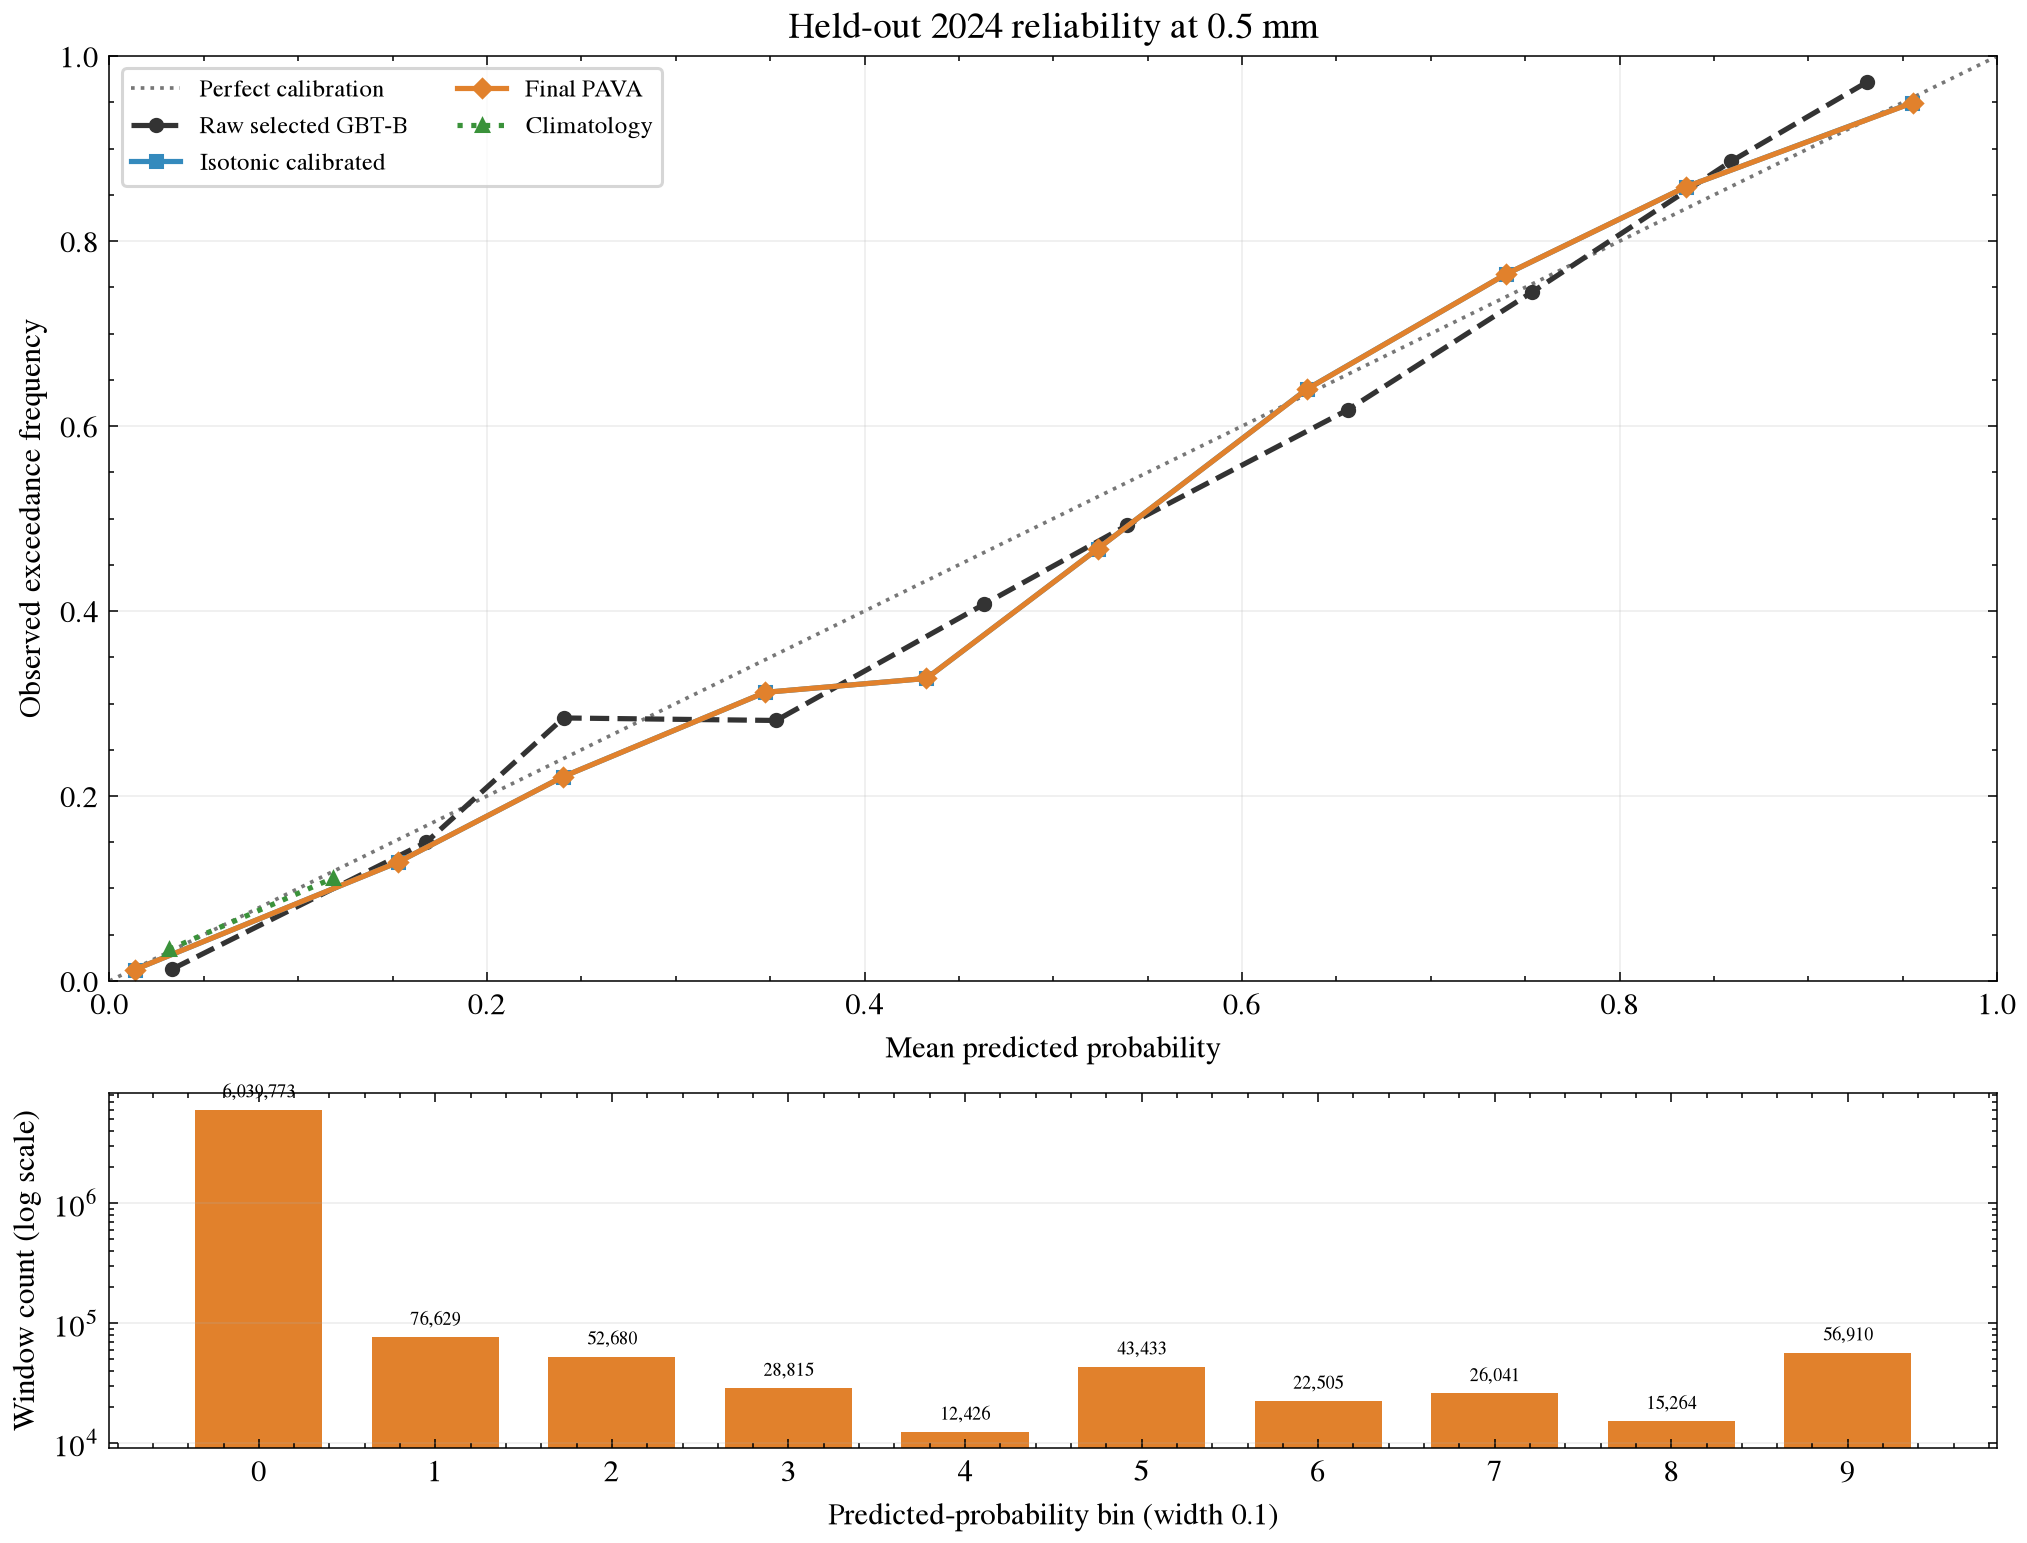
\includegraphics[width=0.9\linewidth]{figures/final/reliability_0.5mm.png}
\caption{Held-out 2024 reliability at the 0.5~mm threshold. Spark's ten
equal-width probability bins are shown for the reliability curve; the lower
panel shows sample counts for the final PAVA bins.}
\label{fig:reliability}
\end{figure}

\begin{figure}[htbp]
\centering
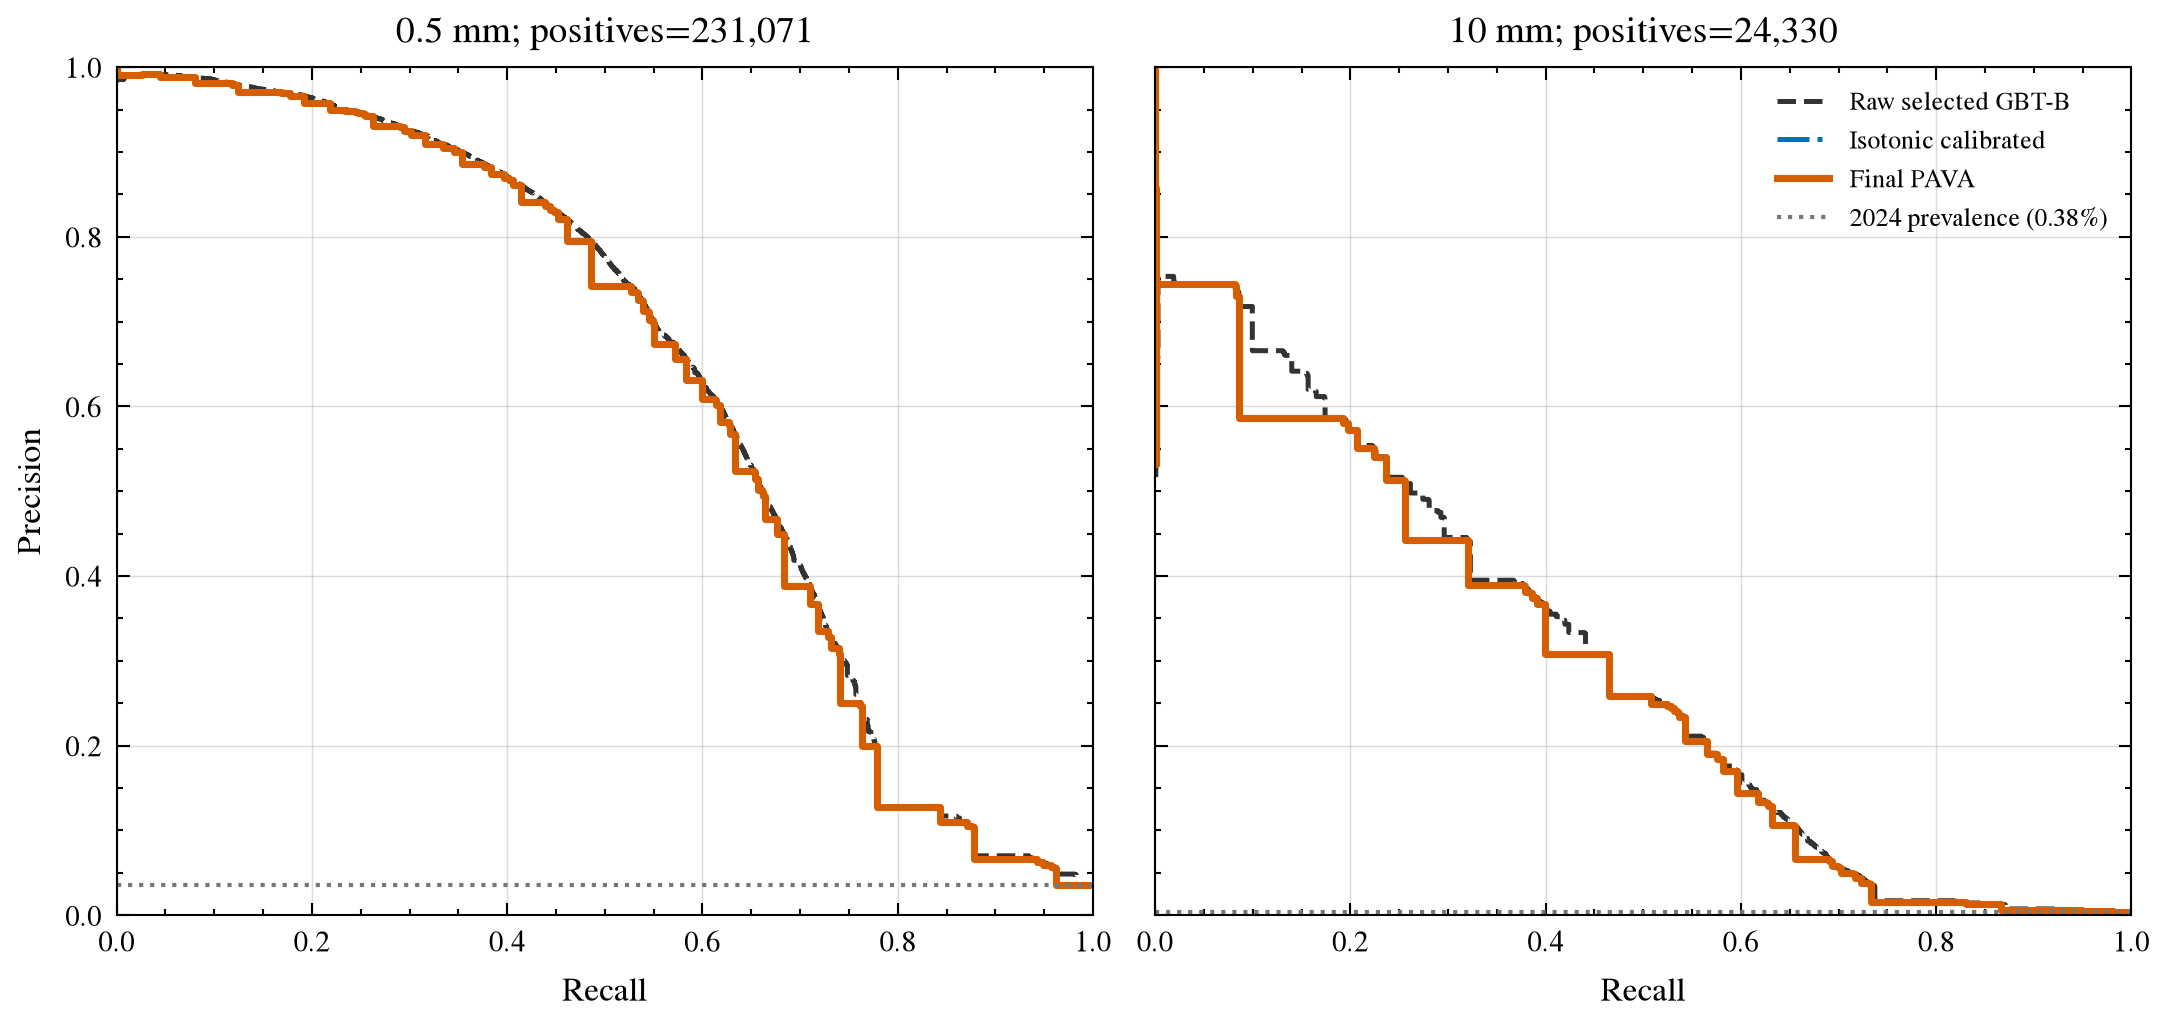
\includegraphics[width=0.96\linewidth]{figures/final/precision_recall_2024.png}
\caption{Threshold-swept precision-recall curves on saved held-out 2024
predictions at 0.5 and 10~mm. Horizontal dotted lines mark the positive
prevalence. PR-AUC values in Table~\ref{tab:test} use Spark's 1,000-bin
evaluator; the plotted curves use the saved scores and
\texttt{precision\_recall\_curve}~\cite{sklearnpr}.}
\label{fig:pr-curves}
\end{figure}

The reliability diagnostics show weighted ECE moving from 0.022701 for raw
scores to 0.001670 after isotonic calibration and 0.0016699 after PAVA; the
climatology value is 0.001425. ECE is aggregated over all stations and periods;
it does not assess calibration within individual stations or months.

\begin{table}[htbp]
\centering\small
\caption{Held-out 2024 metrics at intermediate thresholds obtained by linear
interpolation between the PAVA-projected primary anchors.}
\label{tab:interpolation}
\begin{tabular}{r r r r}
\toprule
Threshold (mm) & PR-AUC & Brier & F1 \\
\midrule
0.30 & 0.6565 & 0.02293 & 0.6126 \\
0.75 & 0.6130 & 0.01751 & 0.5723 \\
1.50 & 0.5435 & 0.01287 & 0.5504 \\
3.50 & 0.4401 & 0.00800 & 0.4529 \\
7.50 & 0.3405 & 0.00435 & 0.3214 \\
\bottomrule
\end{tabular}
\end{table}

Across 53 calendar-week blocks, the paired weekly mean Brier difference
(final PAVA GBT-B minus climatology) was $-0.00877$, with a 95\% bootstrap
interval of $[-0.01091,-0.00669]$ from 1,000 replicates. The one-week block
length was not estimated from the temporal dependence structure.

